\chapter{自动驾驶运行时通信系统测试与分析}
本章在上一章实现了自动驾驶运行时通信系统的各功能模块的基础上,以验证本系统设计的可行性与准确性为目标,展开
对整个自动驾驶运行时通信系统进行功能性测试和非功能性测试。本章从测试环境、测试方法以及测试结果展开论述,并给出测试结果。

\section{测试环境}
本节是对测试环境的介绍,即自动驾驶运行时通信系统的运行环境。本系统支持在兼容Linux的操作系统上运行,并且支持在x86或ARM架构
的CPU上运行。本文测试选用个人笔记本对系统进行测试,具体配置如表6.1所示。
\begin{table}[htb]
  \centering\small
  \caption{测试环境配置}
  \label{tab:exampletable}
  \begin{tabular}{cc}
    \toprule
    硬件 & 配置信息 \\
    \midrule
    操作系统 & Ubuntu16.04.12\\
    处理器 & Intel Core i7-8550U, 1.80GHz $\times$ 8\\
    内存 & 16GB, DDR4 2400MHz\\
    硬盘 & 512GB\\
    \bottomrule
  \end{tabular}
\end{table}
    
\section{功能性测试}
根据需求分析中对通信单元模块和服务模块提出的功能性需求,本节对通信单元模块、服务模块和调度模块展开功能性测试。
\subsection{通信单元模块测试}
对于通信单元模块的测试,编写一个仅包含发布者的任务(test\_pub\_task)和一个仅包含订阅者(test\_sub\_task)的任务,双方以话题/test进行通信,通信数据为C++中的std::string类型,
通信类型使用共享内存进行进程间通信,发布者以20HZ的频率向订阅者发布随机消息。


测试结果如图\ref{pub_sub_test}所示,左侧为发布者所在任务的终端,右侧为订阅者所在任务的终端。从图中可以看出,订阅者全部正确接收到
发布者发布的所有消息。

\begin{figure}[H]
  \centering
  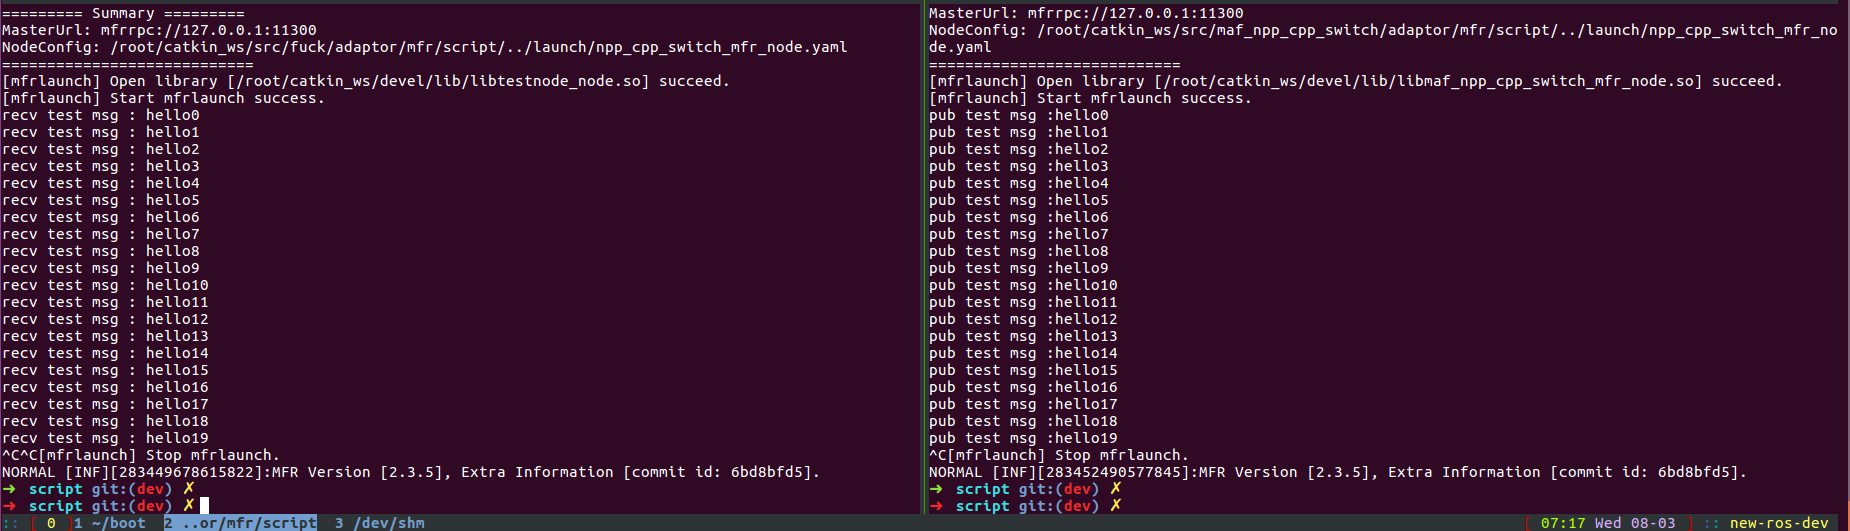
\includegraphics[width=0.95\textwidth]{pub_sub_test.png}
  \caption{通信单元模块测试结果}
  \label{pub_sub_test}
\end{figure}

\subsection{服务模块测试}
对于服务模块的测试,编写一个仅包含一个服务服务端的任务(test\_server\_task)和一个仅包含服务客户端(test\_client\_task)的任务,服务端提供名为/test的回射服务,客户端
向服务端发起请求,服务端将客户端的请求数据返回给客户端。


测试结果如图6.2所示。左侧为服务端所在任务终端,右侧为客户端所在任务的终端。从图中可以看出,服务端正确地返回了客户端的请求数据。
\begin{figure}[H]
  \centering
  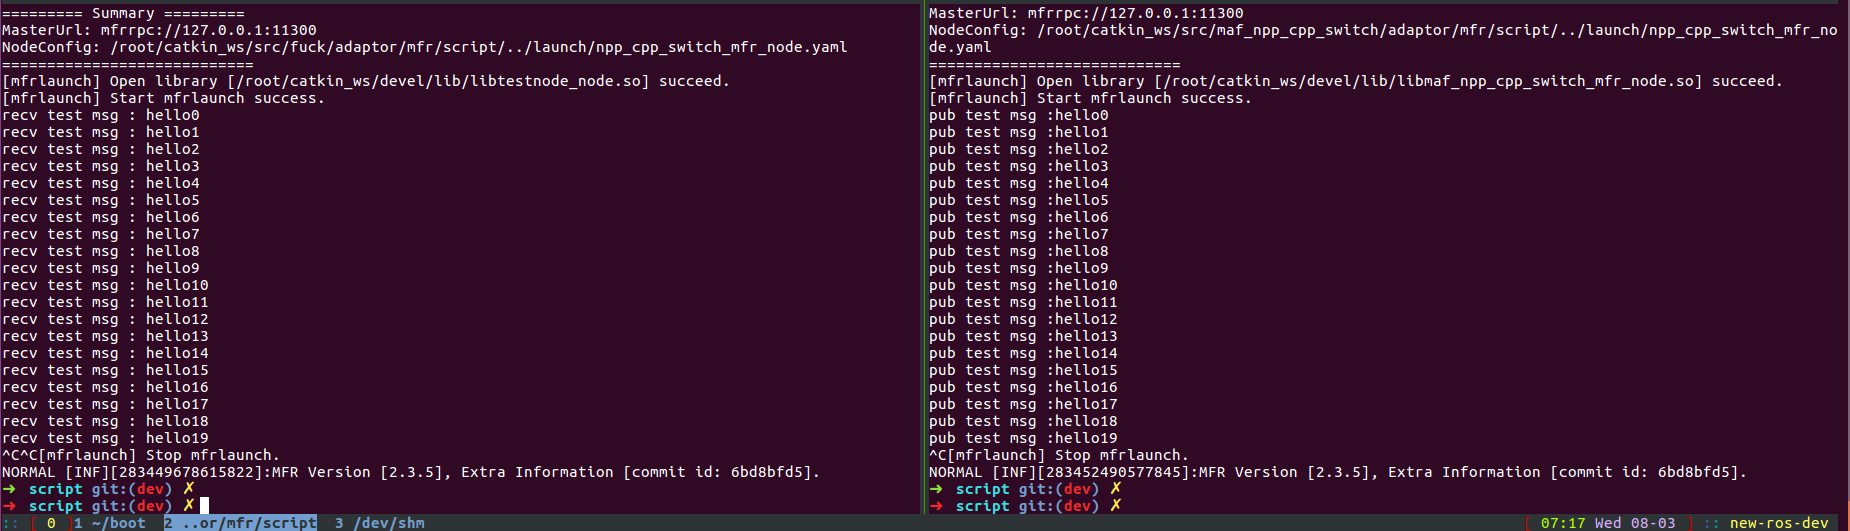
\includegraphics[width=0.95\textwidth]{pub_sub_test.png}
  \caption{服务模块测试结果}
  \label{pub_sub_test}
\end{figure}

\subsection{调度模块测试}
对于调度模块的测试,本节针对其基于时间触发的调度策略进行测试。测试方法为编写一个任务,在任务中设置调度策略为基于时间触发,通过
修改调度频率,记录调度模块对同一个任务调度的时间间隔。
\begin{table}[H]
  \centering\small
  \caption{调度模块测试结果}
  \label{scheduler_test_result}
  \begin{tabular}{cccc}
    \toprule
    调度频率 & 平均时间间隔 & 最小时间间隔 & 最大时间间隔\\
    \midrule
    10HZ & 99.9ms & 99.7ms & 100.3ms \\
    20HZ & 49.8ms & 49.7ms & 50.2ms\\
    50HZ & 19.9ms& 19.7ms & 20.2ms\\
    100HZ & 9.94ms& 9.75ms & 10.21ms\\
    \bottomrule
  \end{tabular}
\end{table}
测试结果如表\ref{scheduler_test_result}所示,基于时间触发的调度策略能够按用户设置的频率周期性调度任务。

\section{非功能性测试}
本系统的非功能性需求同功能性需求一样重要,本节对系统展开非功能性测试,着重于实时性测试。

\subsection{实时性测试}
实时性测试以端到端通信延迟作为衡量指标,测试系统的通信性能。实时性测试以消息大小、发布消息频率和订阅者数量
为变量,全面地对系统的通信性能进行测试。
\subsubsection{消息大小对通信延迟的影响}
本测试场景使用进程间通信的方式,在同一物理机内创建一个发布者和一个订阅者,将本系统共享内存通信(下文统一简写为SHM)、ROS的TCP通信(下文统一简写为ROSTCP)、ROS的UDP通信(下文统一简写为ROSUDP)和百度CyberRT共享内存通信(下文统一简写为CSHM)做通信性能
的对比。本测试固定发布者发布消息频率为10HZ,固定发送500条消息,消息大小分别选用1KB、1MB、4MB和8MB,给出四种通信方式的平均通信延迟、最小通信延迟以及
最大通信延迟。
\begin{table}[htb]
  \centering\small
  \caption{不同大小消息下各通信方式延迟}
  \renewcommand\arraystretch{1.2}
  \label{one_to_one}
  \begin{tabular}{ccccc}
    \toprule
    \multirow{2}{*}{通信方式} & \multirow{2}{*}{消息大小} & \multicolumn{3}{c}{延迟统计}\\
    % \cline{3-5}
     & & 平均延迟 & 最小延迟 & 最大延迟\\
    \midrule
    \multirow{4}{*}{SHM} & 1KB& 0.133935ms& 0.124816ms& 0.259271ms\\ & 1MB & 0.836192ms & 0.672181ms & 0.958912ms \\ & 4MB & 2.394001ms & 2.018293ms & 2.898237ms \\ & 8MB & 4.238182ms & 3.881239ms & 4.791298ms\\
    \hline
    \multirow{4}{*}{ROSTCP} & 1KB& 0.532441ms& 0.264735ms& 0.685397ms\\ & 1MB & 3.258292ms & 2.551780ms & 5.429340ms \\ & 4MB & 11.783733ms & 9.876647ms & 14.62529ms \\ & 8MB & 12.757952ms & 10.384041ms & 17.23690ms\\
    \hline
    \multirow{4}{*}{ROSUDP} & 1KB& 0.515512ms& 0.210117ms& 0.602012ms\\ & 1MB & 10.66662ms & 10.392843ms & 15.690852ms \\ & 4MB & 32.300212ms & 22.969457ms & 41.08326ms \\ & 8MB & 36.016137ms & 25.889108ms & 47.467454ms\\
    \hline
    \multirow{4}{*}{CSHM} & 1KB& 0.126589ms& 0.101587ms& 0.135296ms\\ & 1MB & 0.769871ms & 0.714389ms & 0.897123ms \\ & 4MB & 2.109284ms & 1.91240ms & 2.319872ms \\ & 8MB & 4.129837ms & 3.981398ns & 4.393987ms\\
    \bottomrule
  \end{tabular}
  \note{注:通信延迟数据包含数据序列化耗时}
\end{table}

表\ref{one_to_one}详细列出了各通信方式的通信延迟数据。从表中可以看出当消息大小在1KB时四种通信方式都可以将通信延迟
保证在1ms之内,但当消息大小达到MB级别时基于共享内存的进程间通信方式明显优于基于网络的进程间通信方式。SHM在通信延迟的表现
与CSHM在同一水平上,但SHM的通信延迟波动较CSHM更大。ROSTCP与ROSUDP在传输大数据量的消息时通信延迟明显上升,与SHM差距较大。值得注意的是ROS对于以UDP通信的方式,
单次传输消息大小的上限为1500KB,当实际消息大小超过1500KB时ROS内部将对消息进行分片并且接收时需要再次合并,且序列化与反序列化操作次数
也将增加,故ROSUDP的通信性能比ROSTCP更低。

\subsubsection{发布消息频率对通信延迟的影响}
本场景使用进程间通信的方式,在同一物理机内创建一个发布者和一个订阅者,将SHM、ROSTCP、和CSHM做通信性能对比。
本测试固定消息大小为4MB,固定发送1000条消息,发布频率分别选用10HZ、20HZ和50HZ,给出三种通信方式的平均通信延迟、最小通信延迟以及
最大通信延迟。

\begin{table}[htb]
  \centering\small
  \caption{不同消息发布频率下各通信方式延迟}
  \renewcommand\arraystretch{1.2}
  \label{frequency_test}
  \begin{tabular}{ccccc}
    \toprule
    \multirow{2}{*}{通信方式} & \multirow{2}{*}{频率大小} & \multicolumn{3}{c}{延迟统计}\\
    % \cline{3-5}
     & & 平均延迟 & 最小延迟 & 最大延迟\\
    \midrule
    \multirow{3}{*}{SHM} & 10HZ& 2.429173ms& 2.101929ms& 2.981249ms\\ & 20HZ & 2.310824ms & 2.099812ms & 2.791724ms \\ & 50HZ & 2.258231ms & 1.986102ms & 2.710980ms \\
    \hline
    \multirow{3}{*}{ROSTCP} & 10HZ& 11.984234ms& 9.975642ms& 12.370449ms\\ & 20HZ & 8.958139ms & 4.623674ms & 12.128937ms \\ & 50HZ & 4.362920ms & 3.106624ms & 11.234283ms \\
    \hline
    \multirow{3}{*}{CSHM} & 10HZ& 2.117953ms& 1.889123ms& 2.327153ms\\ & 20HZ & 2.073856ms & 1.908924ms & 2.291289ms \\ & 50HZ & 2.052384ms & 1.886123ms & 2.319872ms \\
    \bottomrule
  \end{tabular}
  \note{注:通信延迟数据包含数据序列化耗时}
\end{table}

表\ref{frequency_test}详细列出了各通信方式的通信延迟数据。从表中可以看出,SHM、ROSTCP和CSHM的通信延迟都随着发布
消息频率的提升而降低,这个情况验证了\cite{9591166}中提到的可能和节能管理或调度模式的原因导致发布频率提升时端到端
的通信延迟反而降低的情况。其中ROSTCP是受发布频率影响最大的通信方式,发布频率从10HZ提升到50HZ后平均通信延迟下降了
65.6\%。而SHM和CSHM两种通信方式的通信延迟并没有ROSTCP明显,CSHM的通信延迟只下降了2\%,SHM则要稍微明显,下降了7\%。
本文通过对CyberRT共享内存机制以及Linux系统中对网络缓冲区的分析,得出CSHM的读写模型基于无锁环形缓冲区实现,
CSHM的读者采用原子变量主动轮询缓冲区,因此CSHM读写不受网络缓冲区刷新策略的影响。而本文提出的SHM读写模型
依赖于网络通信方式通知读者对共享内存进行读取,当发布频率提升时网络缓冲区刷新频次也随之上升,从而造成写者通知
读者读取消息的通知更快地被系统发出。

\subsubsection{订阅者数量对通信延迟的影响}
本场景使用进程间通信的方式,将SHM、ROSTCP和CSHM做通信性能对比。本测试固定消息大小为4MB,固定发送1000条消息,
固定发布频率为10HZ,在同一台物理机内创建一个发布者和四个订阅者,给出三种通信方式的平均通信延迟、最小通信延迟以及
最大通信延迟。

表\ref{multi_subscribers}详细列出了四个订阅者同时订阅一个发布者各通信方式的通信延迟数据。从表中可以看出,ROSTCP
在订阅者数量明显增多的情况下通信延迟明显上升,在本测试场景下,ROSTCP的平均通信延迟达到了一个订阅者时的四倍。而
SHM和CSHM通信延迟上升不明显,测试结果表明在1-N的通信模式下,使用网络通信作为进程间通信的方式在通信延迟方面远远落后于共享内存。
\begin{table}[htb]
  \centering\small
  \caption{四个订阅者订阅消息各通信方式延迟}
  \renewcommand\arraystretch{1.2}
  \label{multi_subscribers}
  \begin{tabular}{ccccc}
    \toprule
    \multirow{2}{*}{通信方式} & \multirow{2}{*}{频率大小} & \multicolumn{3}{c}{延迟统计}\\
    % \cline{3-5}
     & & 平均延迟 & 最小延迟 & 最大延迟\\
    \midrule
    SHM & 10HZ& 2.429173ms& 2.101929ms& 2.981249ms\\ 
    \hline
    ROSTCP & 10HZ& 44.846649ms& 28.584917ms& 64.373177ms\\ 
    \hline
    CSHM & 10HZ& 2.117953ms& 1.889123ms& 2.327153ms\\ 
    \bottomrule
  \end{tabular}
  \note{注:通信延迟数据包含数据序列化耗时}
\end{table}

\subsection{鲁棒性测试}
本文对共享内存发布订阅端崩溃情况和中心节点崩溃情况进行鲁棒性测试,检测系统在发生异常时能否保持通信和恢复通信。
\subsubsection{共享内存机制鲁棒性测试}
对共享内存机制的鲁棒性测试,本测试以任意一个发布者或订阅者异常退出时剩余的通信节点能否继续保持通信为指标。
测试的方法和结果如表\ref{shared_memory_robust}所示,本系统设计的共享内存读写机制能够在发布者或订阅者
崩溃导致异常退出的情况下保持剩余通信节点正常通信。

\begin{table}[H]
  \centering\small
  \caption{共享内存鲁棒性测试}
  \renewcommand\arraystretch{1.2}
  \label{shared_memory_robust}
  \begin{tabular}{ccc}
    \toprule
    测试用例名称 & 测试步骤 & 测试结果 \\
    \midrule
    发布者崩溃 & \makecell[l]{1.创建五个发布者和五个订阅者,\\以话题/test通信;\\2.使用kill -9命令强制终止一个发布者\\所在进程;} & \makecell[l]{1.发布者所在进程立即终止;\\2.互斥锁一致性恢复正常,\\剩余发布者正常发送消息\\3.订阅者能够正常接受消息;}\\
    \hline
    订阅者崩溃 & \makecell[l]{1.创建五个发布者和五个订阅者,\\以话题/test通信;\\2.使用kill -9命令强制终止一个订阅者\\所在进程;} & \makecell[l]{1.订阅者所在进程立即终止;\\2.message slot的readcount被\\发布者恢复;\\3.订阅者能够正常接受消息,\\没有出现message slot全部无\\法获取的情况;} \\
    \bottomrule
  \end{tabular}
\end{table}

\subsubsection{中心节点鲁棒性测试}
对中心节点的鲁棒性测试,本测试以监控脚本能否在中心节点进程异常退出后重启中心节点,并且中心节点被重启后能够从
本地保存的json文件中恢复网络拓扑信息为测试指标。测试的方法和结果如表\ref{master_robust}所示,本系统设计的中心节点异常恢复机制能够在
中心节点异常退出后及时重启并且恢复先前的网络拓扑信息,有效地保证了整个系统的正常通信。

\begin{table}[H]
  \centering\small
  \caption{共享内存鲁棒性测试}
  \renewcommand\arraystretch{1.2}
  \label{master_robust}
  \begin{tabular}{ccc}
    \toprule
    测试用例名称 & 测试步骤 & 测试结果 \\
    \midrule
    发布者崩溃 & \makecell[l]{1.启动中心节点;\\2.使用kill -9命令强制终止中心节点\\所在进程;} & \makecell[l]{1.中心节点所在进程立即终止;\\2.监控脚本检测到中心节点异常\\退出并重启中心节点;\\3.中心节点成功从json文件恢复\\网络拓扑信息;}\\
    \bottomrule
  \end{tabular}
\end{table}

\subsection{可靠性测试}
本系统承担着每个车辆自动驾驶系统所有算法模块的通信任务且自动驾驶系统需要长时间持续运行,
通信系统的可靠性直接影响车辆在自动驾驶时的稳定性和可靠性。本节对整个自动驾驶运行时通信系统进行可靠性测试,测试方法为
手动制作一条包含城区和高架的路线,路线总长度约为20km,自动驾驶车辆连续跑10圈,耗时约为7小时。
测试的步骤和结果如表所示。

\begin{table}[H]
  \centering\small
  \caption{通信系统可靠性测试}
  \renewcommand\arraystretch{1.2}
  \label{master_robust}
  \begin{tabular}{ccc}
    \toprule
    测试用例名称 & 测试步骤 & 测试结果 \\
    \midrule
    通信系统可靠性测试 & \makecell[l]{1.启动自动驾驶车辆;\\2.部署自动驾驶算法软件包;\\3.为自动驾驶车辆选择行驶路线;\\4.通过拨杆使自动驾驶车辆进入\\自动驾驶状态;\\5.跑完10圈路线} & \makecell[l]{通信系统在6小时48分钟的长时\\间运行期间能够保证正常通信。\\}\\
    \bottomrule
  \end{tabular}
\end{table}

\section{本章小结}
本章对自动驾驶运行时通信系统做了详细的测试,包括功能性测试和非功能性测试,对测试环境、测试方法和测试用例做出了详细的介绍。
测试的重点在通信的端到端延迟和鲁棒性,并且将本系统与同类产品进行比较。通过本章的测试结果,表明了自动驾驶
运行时通信系统达到了预期。
